\chapter{Quantum computation of convolution}\label{app:example-quantum-convolution}

Using the quantum convolution algorithm in Algoritm~\ref{alg:qca}, we compute for the convolution of the binary indicator sequences $\text{T}_a=11000100$, $\overline{\text{P}}_a=10000000$ and the sequences $\text{T}_b=00111000$, $\overline{\text{P}}_b=01100000$. The quantum superposition states corresponding to these sequences and computed using the ESQUID sub-routine are the states
\begin{align*}
	\vert \alpha_a \rangle_0 &= \sqrt{\frac{1}{3}}\vert 000 \rangle + \sqrt{\frac{1}{3}}\vert 001 \rangle + \sqrt{\frac{1}{3}}\vert 101 \rangle\ ,\\
	\vert \beta_a \rangle_0 &= \vert 000 \rangle,\\
	\vert \alpha_{b} \rangle_0 &= \sqrt{\frac{1}{3}}\vert 010 \rangle + \sqrt{\frac{1}{3}}\vert 011 \rangle + \sqrt{\frac{1}{3}}\vert 100 \rangle\\
	\vert \beta_{b} \rangle_0 &= \sqrt{\frac{1}{2}}\vert 001 \rangle + \sqrt{\frac{1}{2}}\vert 010 \rangle\
\end{align*}
\begin{example}
First, we compute for the convolution of the sequences $\text{T}_a$ and $\overline{\text{P}}_a$. Step 1 of Algorithm~\ref{alg:qca} will compute for the \textit{QFT} of $\vert \alpha_{a} \rangle_0$,
	\begin{align*}
		\vert \alpha_{a} \rangle_1 &= QFT\vert \alpha_{a} \rangle_0 \\
		&= QFT\left( \sqrt{\frac{1}{3}}\vert 000 \rangle + \sqrt{\frac{1}{3}}\vert 001 \rangle + \sqrt{\frac{1}{3}}\vert 101 \rangle \right)\\
		&= \sqrt{\frac{1}{3}} \cdot QFT\vert 000 \rangle + \sqrt{\frac{1}{3}} \cdot QFT\vert 001 \rangle + \sqrt{\frac{1}{3}} \cdot QFT\vert 101 \rangle \\
		&= \sqrt{\frac{1}{3}} \bigg( \sqrt{\frac{1}{8}} \Big(  w^{0} \cdot \vert 000 \rangle +  w^{0} \cdot \vert 001 \rangle +  w^{0} \cdot \vert 010 \rangle +  w^{0} \cdot \vert 011 \rangle +  w^{0} \cdot \vert 100 \rangle +  w^{0} \cdot \vert 101 \rangle \\
		&\ \ \ \ \ \ \ \ \ \ \ \ \ \ \ \ \ \ \ \ \ +  w^{0} \cdot \vert 110 \rangle +  w^{0} \cdot \vert 111 \rangle \Big) \\
		&\ \ + \sqrt{\frac{1}{8}} \Big( w^{0} \cdot \vert 000 \rangle + w^{1} \cdot \vert 001 \rangle + w^{2} \cdot \vert 010 \rangle + w^{3} \cdot \vert 011 \rangle + w^{4} \cdot \vert 100 \rangle + w^{5} \cdot \vert 101 \rangle\\
		&\ \ \ \ \ \ \ \ \ \ \ \ \ \ \ \ \ \ \ \ \ + w^{6} \cdot \vert 110 \rangle + w^{7} \cdot \vert 111 \rangle \Big)\\
		&\ \ + \sqrt{\frac{1}{8}} \Big( w^{0} \cdot \vert 000 \rangle + w^{5} \cdot \vert 001 \rangle + w^{10} \cdot \vert 010 \rangle + w^{15} \cdot \vert 011 \rangle + w^{20} \cdot \vert 100 \rangle + w^{25} \cdot \vert 101 \rangle\\
		&\ \ \ \ \ \ \ \ \ \ \ \ \ \ \ \ \ \ \ \ \ + w^{30} \cdot \vert 110 \rangle + w^{35} \cdot \vert 111 \rangle \Big)  \bigg)\\
%		&= \sqrt{\frac{1}{3}} \bigg( \sqrt{\frac{1}{8}}\Big( \left( w^{0} + w^{0} + w^{0} \right)\vert 000 \rangle \Big) + \sqrt{\frac{1}{8}}\Big( \left( w^{0} + w^{1} + w^{5} \right)\vert 001 \rangle \Big) \\
%		&\ \ \ \ \ \ \ + \sqrt{\frac{1}{8}}\Big( \left( w^{0} + w^{2} + w^{10} \right)\vert 010 \rangle \Big) + \sqrt{\frac{1}{8}}\Big( \left( w^{0} + w^{3} + w^{15} \right)\vert 011 \rangle \Big) \\
%		&\ \ \ \ \ \ \ + \sqrt{\frac{1}{8}}\Big( \left( w^{0} + w^{4} + w^{20} \right)\vert 100 \rangle \Big) + \sqrt{\frac{1}{8}}\Big( \left( w^{0} + w^{5} + w^{25} \right)\vert 101 \rangle \Big) \\
%		&\ \ \ \ \ \ \ + \sqrt{\frac{1}{8}}\Big( \left( w^{0} + w^{6} + w^{30} \right)\vert 110 \rangle \Big) + \sqrt{\frac{1}{8}}\Big( \left( w^{0} + w^{7} + w^{35} \right)\vert 111 \rangle \Big) \bigg) \\
%		&= \sqrt{\frac{1}{3}} \bigg( \sqrt{\frac{1}{8}} \Big( 3\vert 000 \rangle + \vert 001 \rangle + \left( 1+2i \right) \vert 010 \rangle + \vert 011 \rangle - \vert 100 \rangle + \vert 101 \rangle \\
%		&\ \ \ \ \ \ \ + \left( 1-2i \right) \vert 110 \rangle + \vert 111 \rangle \Big) \bigg)
		&= (0.612372435696) \vert 000 \rangle + (0.204124145232) \vert 001 \rangle \\
		& \quad + (0.204124145232 - 0.408248290464\ i) \vert 010 \rangle + (0.204124145232) \vert 011 \rangle \\
		& \quad - (0.204124145232) \vert 100 \rangle + (0.204124145232) \vert 101 \rangle  \\
		& \quad + (0.204124145232 + 0.408248290464\ i) \vert 110 \rangle + (0.204124145232) \vert 111 \rangle
	\end{align*}
	Following the same procedure for Step 2, $QFT\vert \beta_{a} \rangle_0$ will result to
	\begin{align*}
		\vert \beta_{a} \rangle_1 &= QFT\vert \beta_{a} \rangle_0 \\
		&= QFT\left( \vert 000  \rangle \right) \\
		&= \sqrt{\frac{1}{8}} \Big( w^{0} \cdot \vert 000 \rangle + w^{0} \cdot \vert 001 \rangle  + w^{0} \cdot \vert 010 \rangle + w^{0} \cdot \vert 011 \rangle + w^{0} \cdot \vert 100 \rangle + w^{0} \cdot \vert 101 \rangle \\
		&\ \ + w^{0} \cdot \vert 110 \rangle + w^{0} \cdot \vert 111 \rangle \Big) \\
%		&= \sqrt{\frac{1}{8}} \Big( \vert 000 \rangle + \vert 001 \rangle + \vert 010 \rangle + \vert 011 \rangle + \vert 100 \rangle + \vert 101 \rangle + \vert 110 \rangle + \vert 111 \rangle \Big)\ .
		&= (0.353553390593) \vert 000 \rangle + (0.353553390593) \vert 001 \rangle + (0.353553390593) \vert 010 \rangle \\
		&\quad + (0.353553390593) \vert 011 \rangle + (0.353553390593) \vert 100 \rangle + (0.353553390593) \vert 101 \rangle \\
		&\quad + (0.353553390593) \vert 110 \rangle + (0.353553390593) \vert 111 \rangle
	\end{align*}
	Unitary operator $V_\beta$ is then constructed from $\vert \beta_{a} \rangle_1$ such that
	\begin{align*}
		V_{\beta_{i,i}} &= \frac{\langle i \vert \beta_{a} \rangle_1}{\vert \langle i \vert \beta_{a} \rangle_1 \vert} \\
		&= \frac{\langle i \vert QFT \vert \beta_{a} \rangle_0}{\vert \langle i \vert QFT \vert \beta_{a} \rangle_0 \vert}
	\end{align*}
	Note that application of operation $V_\beta \left( \vert \alpha_{a} \rangle_1 \right)$ in Step 3 is an approximation of the dot multiplication step in the classical convolution algorithm. The resulting unitary matrix for operator $V_\beta$ will be
	\begin{align*}	
		V_\beta &=
		\begin{bmatrix}
			\frac{\langle 0 \vert \beta_{a} \rangle_1}{\vert \langle 0 \vert \beta_{a} \rangle_1 \vert} & 0 & 0 & 0 & 0 & 0 & 0 & 0 \\
			0 & \frac{\langle 1 \vert \beta_{a} \rangle_1}{\vert \langle 1 \vert \beta_{a} \rangle_1 \vert} & 0 & 0 & 0 & 0 & 0 & 0 \\
			0 & 0 & \frac{\langle 2 \vert \beta_{a} \rangle_1}{\vert \langle 2 \vert \beta_{a} \rangle_1 \vert} & 0 & 0 & 0 & 0 & 0 \\
			0 & 0 & 0 & \frac{\langle 3 \vert \beta_{a} \rangle_1}{\vert \langle 3 \vert \beta_{a} \rangle_1 \vert} & 0 & 0 & 0 & 0 \\
			0 & 0 & 0 & 0 & \frac{\langle 4 \vert \beta_{a} \rangle_1}{\vert \langle 4 \vert \beta_{a} \rangle_1 \vert} & 0 & 0 & 0 \\
			0 & 0 & 0 & 0 & 0 & \frac{\langle 5 \vert \beta_{a} \rangle_1}{\vert \langle 5 \vert \beta_{a} \rangle_1 \vert} & 0 & 0 \\
			0 & 0 & 0 & 0 & 0 & 0 & \frac{\langle 6 \vert \beta_{a} \rangle_1}{\vert \langle 6 \vert \beta_{a} \rangle_1 \vert} & 0 \\
			0 & 0 & 0 & 0 & 0 & 0 & 0 & \frac{\langle 7 \vert \beta_{a} \rangle_1}{\vert \langle 7 \vert \beta_{a} \rangle_1 \vert}
		\end{bmatrix}\\
	\end{align*}
Since $ 0.353553390593 = \sqrt{\frac{1}{8}}$ and the norm of any number $x \in \mathbb{R}$ is the square root of the square of its self, 
	\begin{align*}
		\vert x \vert &= \sqrt{x^* x} \\
		&= \sqrt{x^2} \\
		&= x
	\end{align*},
then each entry in the diagonal of the matrix for $V_\beta$ will just be equal to 1,
	\begin{align*}
		\frac{\langle i \vert \beta_{a} \rangle_1}{\vert \langle i \vert \beta_{a} \rangle_1 \vert} &= \frac{\langle i \vert \beta_{a} \rangle_1}{\sqrt{ \left(\langle i \vert \beta_{a} \rangle_1\right)^* \langle 0 \vert \beta_{a} \rangle_1}} \\
		&= \frac{\langle i \vert \beta_{a} \rangle_1}{ \sqrt{ ( \langle i \vert \beta_{a} \rangle_1 )^2} } \\
		&= \frac{\langle i \vert \beta_{a} \rangle_1}{\langle i \vert \beta_{a} \rangle_1} \\
		&= 1
	\end{align*}
for $0 \leq i \leq N+M-2$.
Thus,
	\begin{align*}
%		V_\beta &=
%		\begin{bmatrix}
%			\frac{\sqrt{\frac{1}{8}}}{\big\vert \sqrt{\frac{1}{8}} \big\vert} & 0 & 0 & 0 & 0 & 0 & 0 & 0 \\
%			0 & \frac{\sqrt{\frac{1}{8}}}{\big\vert \sqrt{\frac{1}{8}} \big\vert} & 0 & 0 & 0 & 0 & 0 & 0 \\
%			0 & 0 & \frac{\sqrt{\frac{1}{8}}}{\big\vert \sqrt{\frac{1}{8}} \big\vert} & 0 & 0 & 0 & 0 & 0 \\
%			0 & 0 & 0 & \frac{\sqrt{\frac{1}{8}}}{\big\vert \sqrt{\frac{1}{8}} \big\vert} & 0 & 0 & 0 & 0 \\
%			0 & 0 & 0 & 0 & \frac{\sqrt{\frac{1}{8}}}{\big\vert \sqrt{\frac{1}{8}} \big\vert} & 0 & 0 & 0 \\
%			0 & 0 & 0 & 0 & 0 & \frac{\sqrt{\frac{1}{8}}}{\big\vert \sqrt{\frac{1}{8}} \big\vert} & 0 & 0 \\
%			0 & 0 & 0 & 0 & 0 & 0 & \frac{\sqrt{\frac{1}{8}}}{\big\vert \sqrt{\frac{1}{8}} \big\vert} & 0 \\
%			0 & 0 & 0 & 0 & 0 & 0 & 0 & \frac{\sqrt{\frac{1}{8}}}{\big\vert \sqrt{\frac{1}{8}} \big\vert}
%		\end{bmatrix}\\
		V_\beta &=
		\begin{bmatrix}
			1 & 0 & 0 & 0 & 0 & 0 & 0 & 0 \\
			0 & 1 & 0 & 0 & 0 & 0 & 0 & 0 \\
			0 & 0 & 1 & 0 & 0 & 0 & 0 & 0 \\
			0 & 0 & 0 & 1 & 0 & 0 & 0 & 0 \\
			0 & 0 & 0 & 0 & 1 & 0 & 0 & 0 \\
			0 & 0 & 0 & 0 & 0 & 1 & 0 & 0 \\
			0 & 0 & 0 & 0 & 0 & 0 & 1 & 0 \\
			0 & 0 & 0 & 0 & 0 & 0 & 0 & 1
		\end{bmatrix}
	\end{align*}

In this example, $V_{\beta} = I$ where $I$ is the identity operator. Thus, the operation in Step 3 will be
	\begin{align*}
		\vert \alpha_{a} \rangle_2 &= V_{\beta}\vert \alpha_{a} \rangle_1 \\
		&= I\vert \alpha_{a} \rangle_1 \\
		&= \vert \alpha_{a} \rangle_1 \\
%		&= \sqrt{\frac{1}{3}} \bigg( \sqrt{\frac{1}{8}} \Big( 3\vert 000 \rangle + \vert 001 \rangle + \left( 1+2i \right) \vert 010 \rangle + \vert 011 \rangle - \vert 100 \rangle + \vert 101 \rangle \\
%		&\ \ \ \ \ \ \ + \left( 1-2i \right) \vert 110 \rangle + \vert 111 \rangle \Big) \bigg)
		&= (0.612372435696) \vert 000 \rangle + (0.204124145232) \vert 001 \rangle \\
		& \quad + (0.204124145232 - 0.408248290464\ i) \vert 010 \rangle + (0.204124145232) \vert 011 \rangle \\
		& \quad - (0.204124145232) \vert 100 \rangle + (0.204124145232) \vert 101 \rangle  \\
		& \quad + (0.204124145232 + 0.408248290464\ i) \vert 110 \rangle + (0.204124145232) \vert 111 \rangle
	\end{align*}

Lastly, the operation in Step 4 will apply the unitary operation $QFT^{-1}$ to the state $\vert \alpha_{a} \rangle_2$.
	\begin{align*}
		\vert \alpha_{a} \rangle_3 &= QFT^{-1}\vert \alpha_{a} \rangle_2 \\
		&= QFT^{-1} \bigg( \sqrt{\frac{1}{3}} \bigg( \sqrt{\frac{1}{8}} \Big( 3\vert 000 \rangle + \vert 001 \rangle + \left( 1+2i \right) \vert 010 \rangle + \vert 011 \rangle \\
		&\ \ \ \ \ \ \ - \vert 100 \rangle + \vert 101 \rangle + \left( 1-2i \right) \vert 110 \rangle + \vert 111 \rangle \Big) \bigg) \bigg) \\
		&= \sqrt{\frac{1}{3}} \bigg( \sqrt{\frac{1}{8}} \Big( 3 \cdot QFT^{-1}\vert 000 \rangle + QFT^{-1}\vert 001 \rangle + \left( 1+2i \right) QFT^{-1}\vert 010 \rangle + QFT^{-1}\vert 011 \rangle \\
		&\ \ \ \ \ \ \ - QFT^{-1}\vert 100 \rangle + QFT^{-1}\vert 101 \rangle + \left( 1-2i \right) QFT^{-1}\vert 110 \rangle + QFT^{-1}\vert 111 \rangle \Big) \bigg) \\
		&= \sqrt{\frac{1}{3}} \bigg( \sqrt{\frac{1}{8}} \cdot \sqrt{\frac{1}{8}} \Big( 3 \cdot 8 \cdot \vert 000 \rangle + 0 \cdot \vert 001 \rangle + \left( 1+2i \right) \cdot 0 \cdot \vert 010 \rangle + 0 \cdot \vert 011 \rangle \\
%		&\ \ \ \ \ \ \ - 0 \cdot \vert 100 \rangle + 0 \cdot \vert 101 \rangle + \left( 1-2i \right) \cdot 0 \cdot \vert 110 \rangle + 0 \cdot \vert 111 \rangle \Big) \bigg) \\
%		&= \sqrt{\frac{1}{3}} \bigg( \sqrt{\frac{1}{8}} \cdot \sqrt{\frac{1}{8}} \Big( 8\vert 000 \rangle + 8\vert 001 \rangle + 8\vert 101 \rangle \Big) \bigg) \\
%		&= \sqrt{\frac{1}{3}} \bigg( \frac{1}{8}\Big( 8\vert 000 \rangle + 8\vert 001 \rangle + 8\vert 101 \rangle \Big) \bigg) \\
%		&= \sqrt{\frac{1}{3}} \Big( \vert 000 \rangle + \vert 001 \rangle + \vert 101 \rangle \Big)
		&=  (0.57735026919) \vert 000 \rangle + (0.57735026919 - 1.76762539787e^{-17}\ i) \vert 001 \rangle \\
		& \quad + (1.96261557335e^{-17}) \vert 010 \rangle + (1.76762539787e^{-17}\ i) \vert 011\rangle + (0) \vert 100 \rangle \\
		& \quad + (0.57735026919 - 1.76762539787e^{-17}\ i) \vert 101 \rangle + (1.96261557335e^{- 17}) \vert 110 \rangle \\
		& \quad + (1.76762539787e^{-17}\ i) \vert 111 \rangle
	\end{align*}
Note that $0.57735026919 = \sqrt{\frac{1}{3}}$, $1.76762539787e^{-17} \approx 0$ and $1.96261557335e^{-17} \approx 0$. Thus, the convolution of the binary indicator sequences $\text{T}_a = 11000100$ and $\overline{\text{P}}_a = 10000000$ represented as a superposition quantum state of register $\alpha$ is the state
\[
	\vert \alpha_{a} \rangle_3 = \sqrt{\frac{1}{3}} \Big( \vert 000 \rangle + \vert 001 \rangle + \vert 101 \rangle \Big)
\] 
Each substring $\text{T}_a[j-M-1, j]$ compared to $\text{P}_a = 001$, such that $\text{P}_a[M-1]$ is aligned with $\text{T}_a[j]$, and their corresponding amplitude and probability based from the convolution is summarized in Table~\ref{tab:convolution-a-appendix}.
	\begin{table}[h!]
		\begin{center}
		\begin{tabular}{|| c | c | c | c ||}
			\hline 
			\textit{j} & $\text{T}_b [j-M-1,j]$ & $\langle i \vert \alpha_{a_3} \rangle$ &  $\vert \langle i \vert \alpha_{a_3} \rangle \vert^2$\\
			\hline\hline
				0 & 1	  & $0.57735026919$ & 0.333333333333 \\
			\hline
				1 & 11   & $0.57735026919 - 1.76762539787e^{-17}\ i$ & 0.333333333333\\
			\hline
				2 & 110 & $1.96261557335e^{-17}$ & $3.85185988877e^{-34}$\\
			\hline
				3 & 100 & $1.76762539787e^{-17}\ i$   & $3.12449954721e^{-34}$\\
			\hline
				4 & 000 & 0.0  & 0.0\\
			\hline
				5 & 001 & $0.57735026919 - 1.76762539787e^{-17}\ i$  & 0.333333333333\\
			\hline
				6 & 01   & $1.96261557335e^{-17}$ & $3.85185988877e^{-34}$\\
			\hline
				7 & 1    & $1.76762539787e^{-17}\ i$  & $3.85185988877e^{-34}$\\
			\hline
		\end{tabular}
		\end{center}
		\caption{Comparison result between $\text{T}_a = 110001$ and $P_a = 001$.}
		\label{tab:convolution-a-appendix}
	\end{table}
A probability distribution corresponding to the convolution of $\text{T}_a$ and $\overline{\text{P}}_a$ is shown in Figure~\ref{fig:convolution-a-appendix}.

		\begin{figure}
			\centering
			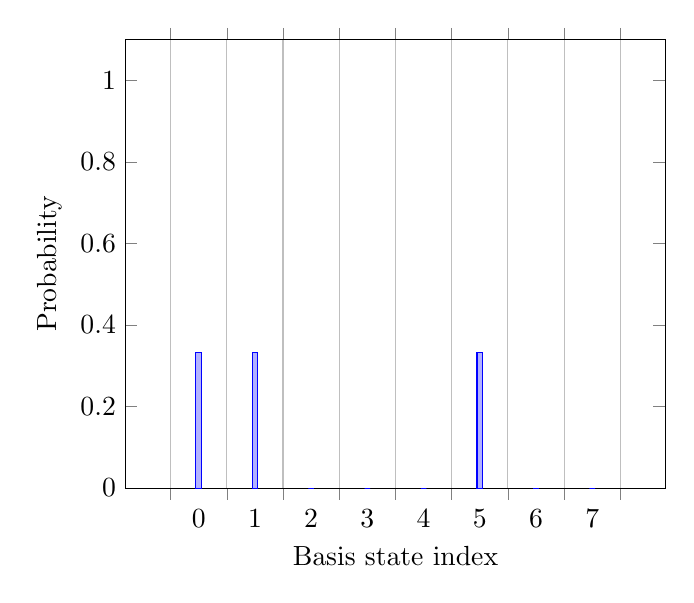
\begin{tikzpicture}
				\begin{axis}[
					ylabel = Probability,
					xlabel = Basis state index,
					ymin = 0,
					ymax = 1.1,
					ybar,
					ybar interval=0.1
				]
				\addplot 
					coordinates {(0,0.333333333333) (1,0.333333333333) (2,0) (3,0) (4,0) (5,0.333333333333) (6,0 ) (7,0) (8,1)};
				\end{axis}
			\end{tikzpicture}
			\caption{Probability distribution for convolution of $\text{T}_a = 11000100$ and $\overline{\text{P}}_a = 10000000$.}
			\label{fig:convolution-a-appendix}
		\end{figure}
	
Again, note that $0.333333333333 = \frac{1}{3}$ and $3.85185988877e^{-34} \approx 0$. Then, the only possible resulting values of a measurement operation on the current state of register $\alpha$ will be the indices 0, 1 and 5. These values correspond to the substrings $\text{T}_a[0, 0] = 1$, $\text{T}_a[0,1] = 11$ and $\text{T}_a[3,5] = 001$.
\end{example}

\begin{example}
\label{exa:aqc-b}
We compute for the convolution of the binary indicator sequences $\text{T}_b$ and $\overline{\text{P}}_b$ given the superposition states $\vert \alpha_b \rangle_0$ and $\vert \beta_b \rangle_0$.
\begin{enumerate}
	\item $\vert \alpha_{b} \rangle_1 = QFT\vert \alpha_{b} \rangle_0 $
		\begin{align*}
			&= QFT \left( \sqrt{\frac{1}{3}}\vert 010 \rangle + \sqrt{\frac{1}{3}}\vert 011 \rangle + \sqrt{\frac{1}{3}}\vert 100 \rangle \right) \\
			&= \left(0.612372435696 \right) \vert 000 \rangle + \left( -0.348461712529 - 0.348461712529\ i \right) \vert 001 \rangle\\
			& \quad + \left( 0.204124145232\ i \right) \vert 010 \rangle + \left( -0.0597865779345 + 0.0597865779345\ i \right) \vert 011 \rangle\\
			& \quad + \left( 0.204124145232 \right) \vert 100 \rangle + \left( -0.0597865779345 - 0.0597865779345\ i \right) \vert 101 \rangle\\
			& \quad + \left( -0.204124145232\ i \right) \vert 110 \rangle + \left( -0.348461712529 + 0.348461712529\ i \right) \vert 111 \rangle
		\end{align*}
	\item $\vert \beta_{b} \rangle_1 = QFT\vert \beta_{b} \rangle_0$
		\begin{align*}
			&= QFT \left( \sqrt{\frac{1}{2}}\vert 001 \rangle + \sqrt{\frac{1}{2}}\vert 010 \rangle \right)\\
			&= \left( 0.5 \right) \vert 000 \rangle + \left( 0.176776695297 - 0.426776695297\ i \right) \vert 001 \rangle\\
			& \quad + \left( -0.25 - 0.25\ i \right) \vert 010 \rangle + \left( -0.176776695297 + 0.0732233047034\ i \right) \vert 011 \rangle\\
			& \quad + \left( 0 \right) \vert 100 \rangle + \left( -0.176776695297 - 0.0732233047034\ i \right) \vert 101 \rangle\\
			& \quad + \left( -0.25 + 0.25\ i \right) \vert 110 \rangle + \left( 0.176776695297 + 0.426776695297\ i \right) \vert 111 \rangle
		\end{align*}
	\item $\vert \alpha_{b} \rangle_2 = V_\beta \vert \alpha_{b} \rangle_1$
		\begin{align*}
			&= V_\beta \Big( \left( 0.5 \right) \vert 000 \rangle + \left( 0.176776695297 - 0.426776695297\ i \right) \vert 001 \rangle\\
			& \quad + \left( -0.25 - 0.25\ i \right) \vert 010 \rangle + \left( -0.176776695297 + 0.0732233047034\ i \right) \vert 011 \rangle\\
			& \quad + \left( 0 \right) \vert 100 \rangle + \left( -0.176776695297 - 0.0732233047034\ i \right) \vert 101 \rangle\\
			& \quad + \left( -0.25 + 0.25\ i \right) \vert 110 \rangle + \left( 0.176776695297 + 0.426776695297\ i \right) \vert 111 \rangle \Big)\\
			&= \left( 0.612372435696 \right) \vert 000 \rangle \\
			& \quad + \left( -0.455287168268 + 0.188586119871\ i \right) \vert 001 \rangle \\
			& \quad + \left( 0.144337567297 - 0.144337567297\ i \right) \vert 010 \rangle \\
			& \quad + \left( 0.0323562628193 - 0.0781149285259\ i  \right) \vert 011 \rangle \\
			& \quad + \left( 0.204124145232\ i \right) \vert 100 \rangle \\
			& \quad + \left( 0.0323562628193 + 0.0781149285259\ i  \right) \vert 101 \rangle\\
			& \quad + \left( 0.144337567297 + 0.144337567297\ i \right) \vert 110 \rangle \\
			& \quad + \left( -0.455287168268 - 0.188586119871\ i \right) \vert 111 \rangle 
		\end{align*}
	\item $\vert \alpha_{b} \rangle_3 = QFT^{-1}\vert \alpha_{b} \rangle_2$
		\begin{align*}
			&= QFT^{-1}\Big( \left( 0.612372435696 \right) \vert 000 \rangle + \left( -0.455287168268 + 0.188586119871\ i \right) \vert 001 \rangle \\
			& \quad + \left( 0.144337567297 - 0.144337567297\ i \right) \vert 010 \rangle \\
			& \quad + \left( 0.0323562628193 - 0.0781149285259\ i  \right) \vert 011 \rangle + \left( 0.204124145232\ i \right) \vert 100 \rangle \\
			& \quad + \left( 0.0323562628193 + 0.0781149285259\ i  \right) \vert 101 \rangle\\
			& \quad + \left( 0.144337567297 + 0.144337567297\ i \right) \vert 110 \rangle \\
			& \quad + \left( -0.455287168268 - 0.188586119871\ i \right) \vert 111 \rangle \Big)\\
			&= (0.0195111123457 + 0.0721687836487\ i ) \vert 000 \rangle \\
			& \quad + (0.0195111123457 - 0.0721687836487\ i) \vert 001 \rangle \\
			& \quad + (-0.074141841541 + 0.0721687836487\ i) \vert 010 \rangle \\
			& \quad + (0.303030398201 - 0.0721687836487\ i) \vert 011 \rangle \\
			& \quad + (0.617625734778 + 0.0721687836487\ i) \vert 100 \rangle \\
			& \quad + (0.617625734778 - 0.0721687836487\ i) \vert 101 \rangle \\
			& \quad + (0.303030398201 + 0.0721687836487\ i) \vert 110 \rangle \\
			& \quad + (-0.074141841541 - 0.0721687836487\ i) \vert 111 \rangle
		\end{align*}
\end{enumerate}
The final state of register $\alpha$ which represents the convolution of the binary indicator sequences $\text{T}_b$ and $\overline{\text{P}}_b$ will be the quantum superposition state $\vert \alpha_{b} \rangle_3$. Each substring $\text{T}_b [j-M-1,j]$ compared to $P_b = 110$ such that $\text{T}_b [j]$ is aligned with $\text{P}_b[M-1]$, and their corresponding basis state's amplitude and probability are shown in Table~\ref{tab:convolution-b-appendix}. A probability distribution corresponding to the convolution of $\text{T}_b$ and $\overline{\text{P}}_b$ is shown in Figure~\ref{fig:convolution-b-appendix}.

	\begin{table}[h!]
	\begin{center}
	\begin{tabular}{|| c | c | c | c ||}
		\hline 
		\textit{j} & $\text{T}_b [j-M-1,j]$ & $\langle i \vert \alpha_{b_3} \rangle$ &  $\vert \langle i \vert \alpha_{b_3} \rangle \vert^2$\\
		\hline\hline
			0 & 0	  & 0.0195111123457 + 0.0721687836487\ i & 0.0055890168383\\
		\hline
			1 & 00   & 0.0195111123457 - 0.0721687836487\ i & 0.0055890168383\\
		\hline
			2 & 001 & -0.074141841541 + 0.0721687836487\ i & 0.0107053460004\\
		\hline
			3 & 011 & 0.303030398201 - 0.0721687836487\ i   & 0.0970357555674\\
		\hline
			4 & 111 & 0.617625734778 + 0.0721687836487\ i  & 0.386669881594\\
		\hline
			5 & 110 & 0.617625734778 - 0.0721687836487\ i   & 0.386669881594\\
		\hline
			6 & 00   & 0.303030398201 + 0.0721687836487\ i  & 0.0970357555674\\
		\hline
			7 & 0    & -0.074141841541 - 0.0721687836487\ i  & 0.0107053460004\\
		\hline
	\end{tabular}
	\end{center}
	\caption{Comparison result between $\text{T}_b = 001110$ and $P_b = 110$.}
	\label{tab:convolution-b-appendix}
	\end{table}

		\begin{figure}
			\centering
			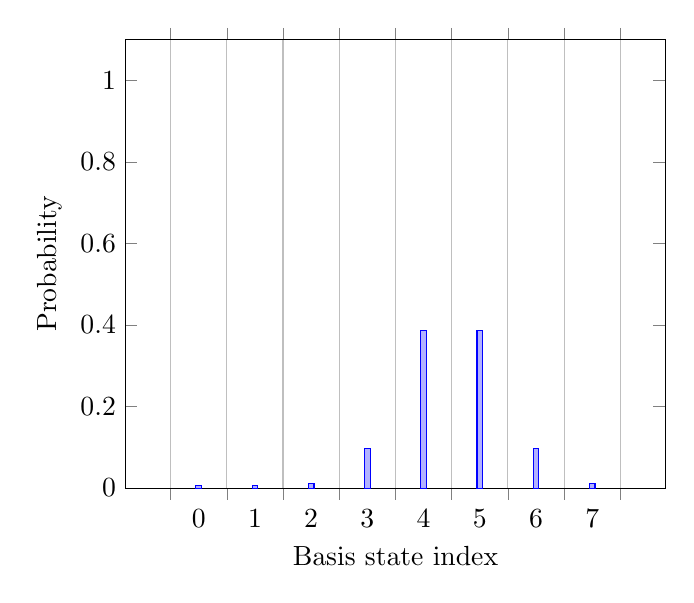
\begin{tikzpicture}
				\begin{axis}[
					ylabel = Probability,
					xlabel = Basis state index,
					ymin = 0,
					ymax = 1.1,
					ybar,
					ybar interval=0.1
				]
				\addplot 
					coordinates {(0,0.0055890168383) (1,0.0055890168383) (2,0.0107053460004) (3,0.0970357555674) (4,0.386669881594) (5,0.386669881594) (6,0.0970357555674 ) (7,0.0107053460004) (8,0)};
				\end{axis}
			\end{tikzpicture}
			\caption{Probability distribution for convolution of $\text{T}_b = 00111000$ and $\overline{\text{P}}_b = 01100000$.}
			\label{fig:convolution-b-appendix}
		\end{figure}

As shown in Table~\ref{tab:convolution-b-appendix} the substrings $\text{T}_b [j-M-1, j]$ with highest probability of occurring from a measurement operation of state of register $\alpha$ are first those for which $j=4$ and $j=5$, followed by those for which $j=3$ and $j=6$, then that for which $j=7$ and $j=2$ and lastly, that for which $j=1$ and $j=0$.
\end{example}
